\section{Fahrzeugführungsebene längs/quer}
\label{ch_Fahrzeugführungsebene}

Im vorangegangenen Abschnitt wurde dargestellt, wie die Trajektorienfolgeregler durch Vorgabe einer Sollkrümmung $\kappa_\mathrm{d}$ und einer Solllängsbeschleunigung $a_{x\mathrm{d}}$ das Fahrzeug auf der geplanten Trajektorie führen. Dieser Abschnitt befasst sich nun mit den Regelungsstrukturen der Fahrzeugführungsebene, die diese Vorgaben durch Ansteuerung der Aktuatoren umsetzten. Dabei müssen eine Reihe von Anforderungen berücksichtigt werden, die sich aus der im Abschnitt \ref{S:Intro} vorgestellten Regelungsaufgabe ergeben. Insbesondere ist die Fahrzeugsführungsebene für Störunterdrückung und Robustheit bezüglich der Fahrzeug- und Aktuatoreigenschaften verantwortlich. Außerdem findet auf dieser Ebene die direkte Interaktion mit dem Fahrer statt, bei der die verschiedenen Kooperationsgrade berücksichtigt werden müssen.

\subsection{Störgrößenbeobachter (Disturbance Observer) - Grundstruktur}\label{subS:DO_Basic}

Die Bewegung des Fahrzeugs unterliegt sowohl in Längs- als auch in Querrichtung nicht vernachlässigbaren Störungen\index{Störung}. Diese müssen durch geeignete Reglerstrukturen in Abhängigkeit des gewünschten Autonomiegrades mehr oder weniger vollständig kompensiert werden.
Ein klassischer I-Anteil wäre dazu prinzipiell in der Lage, bietet aber nicht die notwendigen Freiheitsgrade, sein Störunterdrückungsverhalten an den gewünschten Autonomiegrad anzupassen.

%In die erste Klasse fällt beispielsweise ein klassischer I-Anteil. Dieser ist in der Lage, bestimmte Störungen stationär zu unterdrücken.
%Dabei kann jedoch nur das Zeitverhalten des Ausregelns der Störung nicht aber der zu unterdrückende Anteil der Störung eingestellt werden.
%Für die Anwendung in einer Architektur mit variablem Autonomiegrad liegt in dieser Unnachgiebigkeit ein wesentlicher Grund, weswegen ein klassischer I-Anteil nicht geeignet ist
 
Zum Einsatz kommen daher Störgrößenbeobachter (engl. \emph{disturbance observer}, DO, siehe \cite{Ohnishi1987}) mit gleichzeitiger Kompensation, deren grundlegende Struktur in \refFig{DO_Basic} dargestellt ist. Die Struktur ist augenfällig verwandt mit IMC (engl. \emph{internal model control}, siehe \cite{GarciaMorari82}), welches in \refFig{IMC_Basic} dargestellt ist. Beide Strukturen weisen bei richtiger Wahl der Übertragungsfunktion $Q(s)$ sehr gute Störunterdrückung auf. DO bietet darüber hinaus im Kontext der angestrebten Einstellbarkeit der Störunterdrückung intuitiv nachvollziehbare Eingriffsmöglichkeiten. Außerdem ist das Führungsverhalten bei DO unter der Annahme $G\approx\tilde G$ unabhängig von $Q$ und kann über einen überlagerten Regler getrennt eingestellt werden.


%Lösungen aus der zweiten Klasse haben im Kontext variabler Autonomiegrade den Vorteil, dass die Unterdrückung der Störungen nicht nur hinsichtlich des Zeitverhaltens, sondern auch hinsichtlich des stationären Verhaltens gezielt beeinflusst werden kann. Außerdem ist es damit möglich, Führungs- und Störverhalten der Regelung unabhängig voneinander einzustellen.

%\refFig{DO_allg} zeigt eine mögliche Struktur für einen Störgrößenbeobachter mit gleichzeitiger Kompensation (Störunterdrückung). Diese Struktur hat bereits in vielen regelungstechnischen Anwendungen ihre positiven Eigenschaften unter Beweis gestellt, siehe Literatur.


\begin{figure}[htp!]

\begin{minipage}[t]{0.5\textwidth}
\centering
\import{Bilder/DO_allg/}{DO_Basic_compact.pdf_tex}
\parbox{0.9\textwidth}{\captionof{figure}{Grundstruktur des Störgrößenbeobachters (\emph{disturbance observer}, DO) mit Kompensation}\label{fig:DO_Basic}}
\end{minipage}
\begin{minipage}[t]{0.5\textwidth}
\centering
\import{Bilder/DO_allg/}{IMC_Basic_compact.pdf_tex}
\parbox{0.8\textwidth}{\captionof{figure}{Grundstruktur \emph{internal model control} (IMC)}\label{fig:IMC_Basic}}
\end{minipage}

\end{figure}



In \refFig{DO_Basic} steht $G$ für das dynamische Verhalten einer Reglestrecke, $\tilde G$ ist eine Näherung dieses Verhaltens. Durch die Invertierung von $\tilde G$ im Rückführpfad wird der Ausgang $y$ in eine virtuelle Eingangsgröße $\tilde u$ umgerechnet, die anschließen mit dem tatsächlichen Eingang $u$ verglichen wird. Da die Invertierung von $\tilde G$ üblicherweise nicht realisierbar ist, wird das Tiefpassfilter $Q$ eingeführt, sodass $Q\tilde G$ realisierbar wird. Die damit einhergehende Verzögerung von $\tilde u$ im Vergleich zu $u$ wird beim Vergleich berücksichtigt, indem auch $u$ das Tiefpassfilter $Q$ durchläuft. Die Differenz $Qu-\tilde u$ liefert auf Grundlage dieser Interpretation eine Abschätzung $\tilde d_1$ der Eingangsstörung $d_1$, wobei die Auswirkung von $d_2$ auf den Eingang zurückgerechnet auch berücksichtigt wird. Durch die Rückführung von $-\tilde d_1$ auf den Eingang werden die Störungen $d_1$ und $d_2$ kompensiert.



%Darin ist $G$ die Übertragungsfunktion einer Regelstrecke, für die die Näherung $\tilde G$ existiert. Auf die Strecke wirken verschiedene Störungen, die hier als Eingangsstörung $d_1$ und Ausgangsstörung $d_2$ modelliert sind. Unter der Annahme, dass $\tilde G\approx G$ und zunächst mit der Näherung $Q\approx 1$ kann der Block $Q \tilde G ^{-1}$ wie folgt interpretiert werden: der durch die Störungen $d_1$ und $d_2$ beeinflusste Ausgang $y$ der Strecke wird auf eine virtuelle Eingangsgröße $\tilde u$ so zurückgerechnet, dass $y$ dann der ungestörte Ausgang von $G$ bei Anregung mit $\tilde u$ wäre, wobei $\tilde u$ den Einfluß der Störungen enthält. Subtrahiert man nun $u$ von $\tilde u$ bleibt eine Abschätzung $\tilde d$ für die Wirkung aller Störungen $d_1$ und $d_2$ bezogen auf den Eingang übrig. Wird $\tilde d$ dann wiederum von $u_\mathrm r$ subtrahiert, so werden damit die Störungen $d_1$ und $d_2$ kompensiert.
%
%Da $\tilde G$ im Normalfall nicht invertierbar, $\tilde G^{-1}$ also nicht realisierbar ist, wird das Filter $Q$ eingeführt. Damit $Q \tilde G ^{-1}$ realisierbar wird, muss $Q$ den Nullstellenüberschuss von $\tilde G ^{-1}$ ausgleichen, also Tiefpassverhalten haben. Die damit einhergehende Verzögerung von $\tilde u$ muss auch auf $u$ angewendet werden, bevor die Differenz $\tilde u-Qu$ gebildet wird.

Die Übertragungsfunktionen der Störungen $d_1$ und $d_2$ auf den Ausgang $y$ ergeben sich dann zu 
\begin{equation}
\setlength\arraycolsep{11pt}
\begin{matrix}
G_{d_1\rightarrow y} = \frac{G\tilde G(1-Q)}{\tilde G(1-Q)+GQ}\Biggr\rvert_{Q=1}=0
&
G_{d_2\rightarrow y} = \frac{\tilde G(1-Q)}{\tilde G(1-Q)+GQ}\Biggr\rvert_{Q=1}=0
\end{matrix}
\label{eq:DO1}
\end{equation}

Beide Störübertragungsfunktionen in \refEq{DO1} werden stationär $0$, wenn die stationäre Verstärkung von $Q$ zu 1 gewählt wird. Das dynamische Verhalten der Störunterdrückung ist unter Berücksichtung des Messrauschens $n$ über die Wahl der Pole von $Q$ einstellbar.


Die Verwandschaft des hier eingesetzten Störgrößenbeobachters mit einem klassischen I-Anteil wird offensichtlich, wenn man die linke Rückkopplungschleife im Signalfluss von \refFig{DO_Basic} wie in \refFig{DO_Int} dargestellt umformt.

\begin{figure}[htp!]
\centering
\import{Bilder/DO_allg/}{DO_Int.pdf_tex}
\caption{Rückkopplung des Eingangs $u$ im Störgrößenbeobachter ergibt in der Grundform PI-Verhalten}
\label{fig:DO_Int}
\end{figure}

Ist $Q(s)$ ein Tiefpassfilter der Form
\begin{equation}
Q(s)=\frac{1}{1 + \lambda_1 s + \lambda_2 s^2 + \hdots}
\end{equation}
dann ist die Übertragungsfunktion von $(u_\mathrm r{-}\tilde u)$ zu $u$
\begin{equation}
G_\mathrm{PI}(s)=1+\frac{1}{s(\lambda_1+\lambda_2 s + \hdots)}
\end{equation}
also eine Kombination aus P-Verhalten mit Verstärkung 1 und in Abhängigkeit der Koeffizienten
$\lambda_i$ mehr oder weniger verzögertem I-Verhalten. Folglich verhält sich $u$ im oberen Frequenzbereich wie $u_\mathrm{r}$, im unteren Frequenzbereich wird sich hingegen $u$ so einstellen, dass $u_\mathrm{r}-\tilde u=0$.

Neben der störunterdrückenden Wirkung des Stögrößenbeobachters ist eine weitere Eigenschaft dieser Struktur von großem Vorteil, die zumindest qualitativ offenbar wird, wenn man das Übertragungsverhalten von $u_\mathrm{r}$ nach $y$ für $Q=1$ betrachtet.
\begin{equation}
G_{u_\mathrm{r}\rightarrow y}=\frac{G\tilde G}{\tilde G(1-Q)+GQ}
\Biggr\rvert_{Q=1}=\tilde G\label{eq:DO3}
\end{equation}
\refEq{DO3} bedeutet, dass der Störgrößenbeobachter das Verhalten von $\tilde G$ annimmt. Dies hat zwei Konsequenzen: zum einen ist der Störgrößenbeobachter robust auch bei größeren Abweichungen zwischen dem realen Streckenverhalten und $\tilde G$, zum anderen kann diese Eigenschaft als Entwurfsfreiheitsgrad genutzt werden, um mit $\tilde G$ das Verhalten des störgrößenkompensierten Systems vorzugeben.

Definiert man in Anlehnung an mechanische Systeme die Steifigkeit einer Regelung als Verhältnis der Größe einer Störung (Kraft) zu der durch die Störung verursachten Abweichung vom Nominalverhalten (Verformung), so ergibt sich bei der hier vorliegenden stationär vollständigen Störunterdrückung eine unendlich hohe Steifigkeit bzw. eine Nachgiebigkeit von 0.


%Rechnerisch würde sich mit der Grundstruktur des Störgrößenschätzers aufgrund der genannten Eigenschaften eine stationär unendlich hohe Steifigkeit bezüglich der auftretenden Störungen ergeben.

In den beiden folgenden Abschnitten soll nun gezeigt werden, wie diese hohe Steifigkeit zum einen gezielt reduziert bzw. die Nachgiebigkeit erhöht werden kann und wie es zum anderen gelingt, bestimmte Störungen im Sinne einer Selektivität überhaupt nicht auszuregeln.




%%%%%%%%%%%%%%%%%%%%%%%%%%%%%%%%%%%%%%%%%%%%%%%%%%%%%%%%%%%%%%%%%%%%%%%%%%%%%%%%%%%%%%%%%%

\subsection{Einstellbare stationäre Genauigkeit}\label{subS:DO_Scale_Lim}
Da im Störgrößenbeobachter explizit die beobachtete Störung zunächst ermittelt und dann durch Aufschaltung kompensiert wird, ist es sehr leicht möglich, das Maß der Kompensation einstellbar zu gestalten. Im wesentlichen wird dazu die Struktur aus \refFig{DO_Basic} wie in \refFig{DO_Scale_Lim} dargestellt durch die Möglichkeit einer Skalierung und Begrenzung der aufgeschalteten Störung ergänzt. 

\begin{figure}[htp!]
\centering
\import{Bilder/DO_allg/}{DO_Scale_Lim.pdf_tex}
\caption{Störgrößenbeobachter mit Skalierung und Begrenzung der aufgeschalteten Störung}
\label{fig:DO_Scale_Lim}
\end{figure}

Mit der Skalierung $k$ ändern sich die Störübertragungsfunktionen \refEq{DO1} zu
\begin{equation}
\setlength\arraycolsep{11pt}
\begin{matrix}
G_{d_1\rightarrow y} = \frac{G\tilde G(1-kQ)}{\tilde G(1-kQ)+kGQ} & 
G_{d_2\rightarrow y} = \frac{\tilde G(1-kQ)}{\tilde G(1-kQ)+kGQ}
\end{matrix}\label{eq:DO5}
\end{equation}
Die Auswirkung von $k$ kann unter den Annahmen $Q=1$ und $G\approx\tilde G$ plausibel abgeschätzt werden. \refEq{DO5} vereinfacht sich dann zu
\begin{equation}
\setlength\arraycolsep{11pt}
\begin{matrix}
G_{d_1\rightarrow y}\big\rvert_{Q=1, \tilde G \approx G} = G(1-k) & 
G_{d_2\rightarrow y}\big\rvert_{Q=1, \tilde G \approx G} = (1-k)
\end{matrix}\label{eq:DO7}
\end{equation}

Das bedeutet, dass von der ursprünglichen Auswirkung der Störungen auf den Ausgang $y$ ($Gd_1$ im Falle von $d_1$ und $d_2$ im Falle von $d_2$) ein Anteil $(1-k)$ bleibt bzw. dass nur ein Anteil $k$ der Störungen kompensiert wird, wenn der Störgrößenbeobachter mit einer solchen Skalierung eingesetzt wird.

Mit Ähnlichen Abschätzungen kann die Auswirkung einer Begrenzung im Kompensationspfad greifbar gemacht werden. Darüber hinaus ist die Begrenzung eine wirksame Anti-Windup-Maßnahme, die notwendig ist, wenn die Srecke $G$ im realen System Stellgrößenbegrenzungen enthält.

Im Abschnitt \ref{subS:DO_Delta} wird im Detail vorgestellt, wie Skalierung und Begrenzung eingesetzt werden, um den Störgrößenbeobachter in der Lenkwinkelregelung gezielt nachgiebig  machen.

\subsection{Selektive Kompensation von Störungen}
In diesem Abschnitt wird eine weiter Adaption der Grundstruktur des Störgrößenbeobachters aus Abschnitt \ref{subS:DO_Basic} vorgestellt, die den Störgrößenbeobachter ausgewählten Störungen gegenüber blind macht, d.h., das Übertragungsverhalten dieser Störungen auf den Ausgang unbeeinflusst lässt.
%
Dies gelingt unter der Voraussetzung, dass eine zusätzliche Meßgröße $y_1$ innerhalb der Regelstrecke, z.B. am Ausgang des Aktuators, abgegriffen werden kann, welche nur die Störungen enthält, die zu ignorieren sind. Der Streckenausgang $y$ enthält alle Störungen, siehe \refFig{DO_Modified}.
Der Vergleich von $y_1$ und dem durch die Inverse der Teilstrecke $G_2$ zurückgerechnete Ausgang liefert nun ein Maß $\tilde d_{12}$ nur für die Störungen $d_{12}$ und $d_{22}$ an der Teilstrecke $G_2$. Durch Multiplikation mit $G_1^{-1}$ wird daraus ein auf den Eingang der Strecke umgerechneter Wert $\tilde d$, der bei Aufschaltung die Wirkung der Störungen
$d_{12}$ und $d_{22}$ kompensiert, die Störungen $d_{11}$ und $d_{21}$ jedoch ignoriert.
Wie im Falle der Grundstruktur des Störgrößenbeobachters werden Tiefpaßfilter $Q_1$ und $Q_2$ mit stationärer Verstärkung $1$ benötigt, um das Invertieren der Strecke realisierbar zu machen und um das dynamische Verhalten des Beobachters auszulegen.

\begin{figure}[htp!]
\centering
\import{Bilder/DO_allg/}{DO_Selective.pdf_tex}
%\import{Bilder/DO_allg/}{DO_Modified.pdf_tex}
\caption{Grundstruktur eines selektiven Störgrößenbeobachters zur Kompensation der Störungen $d_{12}$ und $d_{22}$.}
\label{fig:DO_Modified}
\end{figure}

Die Störübertragungsfunktionen sind dann für $Q_1=1$ und $Q_2=1$ (stationär und unterer Frequenzbereich)
\begin{equation}
\begin{matrix*}[l]
G_{d11}&=&G_1 G_2 \tilde G_1 \tilde G_2 \cdot D^{-1} & \hspace{6pt} &
G_{d12}&=&G_2 \tilde G_2 (\tilde G_1 - G_1) \cdot D^{-1} \\
G_{d21}&=&G_2 \tilde G_1 \tilde G_2 \cdot D^{-1}& \hspace{6pt} &
G_{d22}&=&\tilde G_2 (\tilde G_1 - G_1) \cdot D^{-1}
\end{matrix*}
\label{eq:DoSel01}
\end{equation}

mit dem gemeinsamen Nenner $D=\tilde G_2(\tilde G_1 - G_1)+G_1 G_2$.
Es ist leicht zu erkennen, dass die Bedingung $\tilde G_1=G_1$ in den relevanten Frequenzbereichen erfüllt sein muss, damit die Störungen $d_{12}$ und $d_{22}$ dort vollständig kompensiert werden. Mit dieser Bedingung vereinfacht sich \refEq{DoSel01} zu
\begin{equation}
\begin{matrix*}[l]
G_{d11}\bigr\rvert_{\tilde G_1 = G_1}&=&G_1 \tilde G_2 & \hspace{12pt} &
G_{d12}\bigr\rvert_{\tilde G_1 = G_1}&=&0\\
G_{d21}\bigr\rvert_{\tilde G_1 = G_1}&=&\tilde G_2 & \hspace{12pt} &
G_{d22}\bigr\rvert_{\tilde G_1 = G_1}&=&0
\end{matrix*}
\label{eq:DoSel02}
\end{equation}

$d_{11}$ und $d_{21}$ behalten also im wesentlichen das selbe Übertragungsverhalten auf den Ausgang $y$ wie ohne den Störgrößenbeobachter. $d_{12}$ und $d_{22}$ werden ausgeregelt.
 
Die Übertragungsfunktion $G_{u_\mathrm{r}\rightarrow y}$ ist gleich $G_{d11}$ und damit ebenfalls $G_1\tilde G_2$. Es kann also auch bei dieser Form des Störgrößenbeobachters ein Teil des Streckenverhaltens durch die Wahl von $\tilde G_2$ vorgegeben werden bzw. ist dieser Störgrößenbeobachter ebenfalls robust gegenüber Abweichungen zwischen $\tilde G_2$ und $G_2$.
$\tilde G_1$ muss hingegen mit $G_1$ sehr gut übereinstimmen.



%%%%%%%%%%%%%%%%%%%%%%%%%%%%%%%%%%%%%%%%%%%%%%%%%%%%%%%%%%%%%%%%%%%%%%%%%%%%%%%%%%%%%%%%%%%

\subsection{Störgrößenbeobachter Krümmung}\label{subS:DO_Kappa}
Ziel des Krümmungs-Störgrößenbeobachters $\mathrm{DO}_\kappa$ ist es, die gegebene Sollkrümmung der Bahnführungsebene $\kappa_\mathrm{d}$ stationär genau umzusetzen.  Dabei sollen sämtliche Seitenkraftstörungen, die auf das Fahrzeug wirken unterdrückt werden.  Diese können von Seitenwinden,  hängenden Fahrbahnen etc. verursacht werden.  Die Herausforderung dabei ist es, bei kooperativen Kundenfunktionen die Fahrereingriffe nicht als Störung zu unterdrücken um ein nachgiebiges Reglerverhalten darstellen zu können.  Wie im vorangegangen Abschnitt bereits dargestellt, kann die Struktur des selektiven Störgrößenbeobachters unter Rückführung einer Hilfsgröße diesen Zielkonflikt auflösen.  

Zur Beeinflussung der Querdynamik wird im Folgenden nur von Beeinflussung der Vorderachslenkung ausgegangen, sodass die Control Allocation $\mathrm{CA}_\kappa$ entfällt.  Mittels der angenommenen stationären Verstärkung $\tilde k_\kappa$ kann die Sollkrümmung zur Ansteuerung der Lenkwinkelregelung in einen Solllenkwinkel $\delta_\mathrm{d}$ umgerechnet werden:
\begin{equation}
\delta_\mathrm{d} = \tilde k_\kappa^{-1} \kappa_{\delta\mathrm{d}}
\end{equation}
Als Modell für den Entwurf des Störgrößenbeobachters dienen die Gleichungen (\ref{eq:GL2}) und (\ref{eq:Gkappa}).  Dementsprechend ergibt sich die Krümmung als Folge des Übertragungsverhaltens der geregelten Lenkung $G_\delta$ und des Einspurmodells $G_\kappa$.  
%Als Hilfsgröße wird dazu der gemessene Lenkwinkel $\delta$ mittels der Ackermann-Verstärkung umgerechnet: 
%\begin{equation}
%\kappa_\delta = K_{Ackermann} \delta
%\end{equation}
%$\kappa_\delta$ gibt somit die Krümmung wieder die das Fahrzeug bei Abwesenheit von Störungen stationär einnimmt.  Diese wird im Störgrößenbeobachter mit der gemessen Ist-Krümmung verglichen.
Als Hilfsgröße wird der gemessene Lenkwinkel $\delta$ zurückgeführt.  Dieser gibt sowohl das gestellte Moment der unterlagerten Lenkwinkelregelung als auch das Fahrerlenkmoment $\tau_{\delta,\mathrm{drv}}$ wider.  Die auf das Fahrzeug wirkenden und zu unterdrückenden Seitenkraftstörungen $z_\kappa$ sind dagegen nur in der gemessenen Krümmung $\kappa$ sichtbar.  Abb.~\ref{fig:DO_kappa} zeigt die Umsetzung des Krümmungs-Störgrößenbeobachters im Blockschaltbild.  Dessen Ausgang ergibt sich zu:
\begin{equation}
\kappa_\mathrm{do} = \tilde k_\kappa Q_\delta \tilde G_\delta^{-1} \left( Q_\kappa \delta - Q_\kappa \tilde{G}_\kappa^{-1} \kappa \right)
\end{equation}
Die gesamte Stellgröße $\kappaDPrime$ berechnet sich als Summe von $\kappa_\mathrm{d}$ und $\kappa_\mathrm{do}$.  Zur Realisierung der Invertierungen der angenommenen Übertragungsfunktionen $\tilde G_\delta$ und $\tilde G_\kappa$ sind die Tiefpassfilter $Q_\delta$ und $Q_\kappa$ notwendig.  
%
\begin{figure}[ht]
	\centering
	\includegraphics{Bilder/DO_allg/DO_kappa.eps}
	\caption{Selektiver Störgrößenbeobachter auf Krümmungsebene zur Kompensation der Störung $z_\kappa$ ohne Kompensation des Fahrerhandmoments $\tau_{\delta,\mathrm{drv}}$}
	\label{fig:DO_kappa}
\end{figure}
%
Störungen $z_\kappa$ werden mit dieser Struktur stationär genau unterdrückt, wohingegen Fahrerinteraktionen nicht als Störungen interpretiert und ausgeregelt werden.  Auch Anti-Wind-Up Maßnahmen für etwaige Limitierung der Stellgrößen im Aktuator sind nicht notwendig da der  gemessene Lenkwinkel $\delta$ im Gegensatz zur Stellgröße $\delta_\mathrm{d}$ bereits die Limitierung enthält. Der über den Störgrößenbeobachter geschlossene Regelkreis prägt näherungsweise das nominelle Übertragungsverhalten 
\begin{equation}
\tilde G_{\kappa_\mathrm{d}\rightarrow \kappa} \approx \tilde k_\kappa^{-1} \tilde G_\delta \tilde G_\kappa
\end{equation}
auf.  Parameterschwankungen können so beherrscht und die Übertragungsfunktion für den Entwurf der Trajektorienfolgergelung innerhalb der Bahnführungsebene genutzt werden.
%
\subsection{Störgrößenbeobachter Längsbeschleunigung}
Analog zur Krümmungsregelung wird der Entwurf der Längsregelung durchgeführt: Mittels eines Störgrößenbeobachters wird die stationär genaue Umsetzung der Sollbeschleunigung $\aXD$ sichergestellt.  Auch hier wird durch Rückführung einer Hilfsgröße erreicht, dass Fahrerinteraktionen nicht als Störungen unterdrückt werden.  Dazu wird das sich einstellende Summenradmoment $\tau_{x}$ benutzt.  Dieses stellt sich in Folge der Fahrermomente über Gas- und Bremspedal und den Vorgaben durch die Funktion ein.  Als Modell für den Entwurf dient das angenommen Übertragungsverhalten entsprechend Gleichung (\ref{eq:GLong}) und (\ref{eq:Gwhl}).  Die geforderte Sollbeschleunigung wird über die angenommen Fahrzeugparameter $\tilde m$ und $\tilde r$ in ein Sollradmoment umgerechnet:
\begin{equation}
\tau_{x\mathrm{d}} = \aXD \tilde m \tilde r
\end{equation}
$\tilde m$ und $\tilde r$ stehen als Messgrößen im Fahrzeug zur Verfügung und werden durch Schätzverfahren ermittelt.  Die Verteilungslogik auf Antrieb und  Bremse ($\mathrm{CA}_x$) weißt durch im nächsten Abschnitt vorgestellte Logik näherungsweise das Übertragungsverhalten 1 auf und wird deswegen im Entwurf des Störgrößenbeobachters vernachlässigt.

Abb. \ref{fig:DO_acceleration} zeigt die Umsetzung des selektiven Störgrößenbeobachters zur Unterdrückung der Störungen $z_{a_x}$.  Die Stellgröße berechnet sich zu
\begin{equation}
a_\mathrm{x,do} = Q_{\tau_x} \left(\tilde m \tilde r\tilde G_{\tau_x}\right)^{-1} \left( Q_{a_x} \tau_{a_x} - Q_{a_x} \tilde{G}_{a_x}^{-1} a_x \right).
\end{equation}
Zur Realisierung der Invertierungen der angenommenen Übertragungsfunktionen $\tilde G_{\tau_x}$ und $\tilde G_{a_x}$ sind zwei Filter $Q_{\tau_x}$ und $Q_{a_x}$ notwendig.  Der so geschlossene Regelkreis verhält sich näherungsweise wie
\begin{equation}
\tilde G_{a_\mathrm{x,d}\rightarrow a_x} \approx \tilde m \tilde r\tilde G_{\tau_x}  \tilde G_{a_x}.
\end{equation}
% 
Störungen $z_{a_x}$ werden kompensiert,  wohingegen das Fahrerantriebsmoment $\tau_\mathrm{mot,drv}$ und Fahrerbremsmoment $\tau_\mathrm{brk,drv}$ nicht unterdrückt werden.
\begin{figure}[ht]
	\centering
	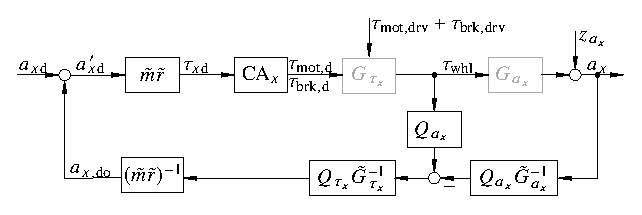
\includegraphics{Bilder/DO_allg/do_acceleration.eps}
	\caption{Selektiver Störgrößenbeobachter auf Beschleunigungsebene zur Kompensation der Störung $z_a$ ohne Kompensation des Fahrermoments $\tau_\mathrm{mot,drv}$ und $\tau_\mathrm{brk,drv}$}
	\label{fig:DO_acceleration}
\end{figure}


%%%%%%%%%%%%%%%%%%%%%%%%%%%%%%%%%%%%%%%%%%%%%%%%%%%%%%%%%%%%%%%%%%%%%%%%%%%%%%

\subsection{Kooperativer Lenkwinkelregler mit Störgrößenbeobachter}\label{subS:DO_Delta}

Der Lenkwinkelregler, C\sus{$\delta$} in \refFig{LongLatOverview}, hat in der Fahrzeugquerführung die Aufgabe, den angeforderten Solllenkwinkel $\delta_\mathrm{d}$ umzusetzen. Dabei soll er je nach Kundenfunktion mehr oder weniger steif sowohl auf Störungen durch den Fahrer $\tau_{\delta,\mathrm{drv}}$ als auch auf äußere und innere Kräfte, die am Lenksystem auftreten, reagieren.

Das Problem, einem geregelten System eine definierte Steifigkeit bzw. Nachgiebigkeit zu verleihen, ist aus der Robotik bekannt und wird dort durch verschiedene Ansätze zur Impedanzregelung gelöst. Dabei lassen sich vereinfacht vier Grundstrukturen identifizieren:
\begin{enumerate}
\item die gewünschte Impedanz des Systems wird beim Entwurf durch die Wahl der Verstärkungsfaktoren realisiert (kommt ohne Kraftsensorik aus)\label{ImpCtrl1}
\item steife Positionsregelung mit überlagertem Admittanzmodell der gewünschten Systemdynamik (Admittanzarchitektur)
\item steife Kraftregelung mit überlagertem Impedanzmodell der gewünschten Systemdynamik (Impedanzarchitektur)
\item kombinierte Positions-/Kraftregelung im Sinne einer Mehrgößen- oder Zustandsregelung
\end{enumerate}

Der hier vorgeschlagene Lenkwinkelregler bedient sich bei diesen Ideen, um der Forderung nach einstellbarer Steifigkeit und stationärer Genauigkeit gerecht zu werden. Dabei tritt das Lenksystem, welches über den Drehstab mit dem Fahrer interagiert, an die Stelle eines Roboters, der über einen Kraftsensor mit seiner Umgebung interagiert.

Im wesentlichen besteht der Lenkwinkelregler aus zwei kaskadierten P-Reglern, $k_{\delta\mathrm{P}}$ und $k_{\delta\mathrm{D}}$ mit Vorsteuerung, deren Strecke das durch einen Störgrößenbeobachter nach \ref{subS:DO_Scale_Lim} störgrößenkompensierte Lenksystem ist, siehe \refFig{Zff}.


\begin{figure}[htp!]
\centering
\import{Bilder/Zff/}{Zff.pdf_tex}
\caption{Kooperativer Lenkwinkelregler mit Störgrößenbeobachter; Steifigkeit und stationäre Genauigkeit sind über die Signale $\eta$ und $\zeta$ einstellbar}
\label{fig:Zff}
\end{figure}


Als Streckenmodell $\tilde G$ kommt im Störgrößenbeobachter das Lenkungsmodell~1 ($G_{\tau\delta}$) zum Einsatz, welches in Abschnitt~\ref{subS:SteeringModels} eingeführt wurde.

Die Reglerparameter, welche Einfluß auf Steifigkeit und stationäre Genauigkeit haben, können von außen durch die Signale $\eta$ (Steifigkeit) und $\zeta$ (stationäre Genauigkeit) verändert werden.
Dieser Eingriff in die Reglerparameter entspricht in seinen Grundzügen der Variante \ref{ImpCtrl1} der Impedanzregelung. Durch die gewählte Reglerstruktur ist es beim Regler aus \refFig{Zff} jedoch möglich, Steifigkeit und stationäre Genauigkeit in Grenzen \emph{unabhängig} voneinander einzustellen.

Die Ansätze zur Impedanzregelung mit Kraftrückführung erfordern i.A. sehr hohe Reglerbandbreiten, da das Übertragungsverhalten von den Stellmomenten zur gemessenen Reaktionskraft typischerweise hohe Bandbreiten aufweist. Je nach Partitionierung des Reglers können diese Reglerbandbreiten im Fahrzeug eventuell nicht realisiert werden. Dennoch ist eine Rückführung des Fahrerhandmomentes $\tau_{\delta\mathrm{,drv}}$, welches teilweise eine passive Reaktion darstellt, erforderlich, wenn sich der Regler steif bzgl. aller Störungen jedoch nachgiebig bzgl. des Fahrers verhalten soll. Die hier vorgeschlagene Lösung entkoppelt das Stellmoment $\tau_{\delta\mathrm{d}}$ und das Reaktionsmoment $\tau_{\delta\mathrm{,drv}}$ (Fahrerhandmoment) in den relevanten Frequenzbereichen indem abhängig von $\tau_{\delta\mathrm{,drv}}$ jedoch zeitlich verzögert die verschiedenen Regleranteile reduziert werden. Dabei sind die Eingriffsschwellen und das Ausmaß der Reduktion wiederum von der gewünschten Steifigkeit $\eta$ abhängig.


%\begin{figure}[htp!]
%\centering
%\import{Bilder/ImpedanceAdmittance/}{impedance_control.pdf_tex}
%\caption{Impedanzarchitektur}
%\label{fig:ImpArch}
%\end{figure}


%%%%%%%%%%%%%%%%%%%%%%%%%%%%%%%%%%%%%%%%%%%%%%%%%%%%%%%%%%%%%%%%%%%%%%%%%%%%%%%%%%
\subsection{Ansteuerung Antrieb und Bremse}
Die Strategie zur (funktionsunabhängigen) Verteilung des Sollradmoments $\tauXDPrime$ auf die beiden Aktuatoren Antrieb und Bremse wird im Folgenden zunächst für den Fall ohne Fahrerinteraktion erläutert: 

Für das Sollantriebsmoment $\tau_\mathrm{mot,d}$ wird direkt das berechnete Sollmoment $\tauXDPrime$ verwendet: 
\begin{equation}
\tau_\mathrm{mot,d}=  \tauXDPrime.
\end{equation}
Zur Ansteuerung der Bremse wird dagegen eine Fallunterscheidung nach der Höhe des zurückgemeldeten zur Verfügung stehenden Schleppmoments $\tau_\mathrm{mot,min}$ durchgeführt:
\begin{equation}\label{eq:pka_bremse}
\tau_\mathrm{brk,d}=\begin{cases} 
0 & \text{falls } \tauXDPrime \geq \tau_\mathrm{mot,min}\\
\tauXDPrime -  \tau_\mathrm{mot,min} & \text{falls }  \tauXDPrime < \tau_\mathrm{mot,min}
\end{cases}
\end{equation}
Dies ist notwendig um den gesamten Stellbereich des Antriebs auszunutzen.  Dieser ist durch das Schleppmoment im Stande, leichte Verzögerungen umzusetzen. Mit der Fallunterscheidung wird vermieden, dass eine negative Sollbeschleunigung automatisch zur Ansteuerung der Bremse führt.

Zur Berücksichtigung des Fahrers wird gewöhnlich das Maximum aus vom geforderten Fahrermoment und Moment der Funktion priorisiert,  sodass der Fahrer die Funktion stets übersteuern kann.  Im Fall von Bremsanforderungen wird dagegen bei Komfortfunktionen wie ACC die automatisierte Längsführung abgeschaltet sobald ein Fahrerbremsmoment angefordert wird. Lediglich bei Sicherheitsfunktionen wie Notbremsassistenten wird das Minimum aus Fahrerbremsanforderung $\tau_\mathrm{brk,drv}$ und der Anforderung der Fahrerassistenzfunktion priorisiert $\tau_\mathrm{brk,d}$. So wird sichergestellt dass stets der höhere Verzögerungswunsch umgesetzt wird.

\FloatBarrier
